\documentclass[11pt]{article}
\usepackage{fontspec}
\setmainfont{Times New Roman}
\usepackage{amsmath,amssymb}
\usepackage[margin=2.3cm]{geometry}
\usepackage{booktabs,graphicx,xcolor}
\usepackage{hyperref}
\hypersetup{colorlinks=true,urlcolor=blue}
\sloppy

\hypersetup{pdftitle={Теңүдемелі түзу сызықты қозғалыс},pdfsubject={PhysLab study guide, content canonical v2 (7d85de57), lang kk},pdfauthor={PhysLab},pdflang={kk}}
\begin{document}
{\small\color{gray} PhysLab / ЕНТ • ҰБТ / Қазақша \quad конспект v2 \quad мазмұн canonical v2 (7d85de57)}

\section*{Теңүдемелі түзу сызықты қозғалыс}
\subsection*{Мақсат}
Видео соңында оқушы бастапқы жылдамдық, үдеу және уақыт бойынша теңүдемелі дененің жылдамдығы мен орын ауыстыруын есептеп, жауапты v(t) графигі астындағы ауданмен тексере алады.

\subsection*{Негізгі мәселе}
Егер жылдамдық өзгермесе — қозғалыс бірқалыпты: v тең s бөлінген t.

Бізде жылдамдық өседі — бірақ әр секундта бірдей шамаға өседі.

Әр секундта жылдамдық секундына үш метрге артады — бұл үдеудің үшке тең екенін білдіреді.

Мұндай қозғалыс теңүдемелі деп аталады.

Жылдамдықтың өсу шапшаңдығын үдеу көрсетеді: a тең жылдамдық өзгерісін уақытқа бөлгенге.

Өлшем бірлігі — метр секундына квадрат.

Икс осін қозғалыс бағытымен бағыттаймыз: алға бағытталғанның бәрі плюс таңбасымен.

Кез келген сәттегі жылдамдық — бастапқы жылдамдық пен өсімшенің қосындысы.

Өсімше — үдеу мен уақыттың көбейтіндісі: v тең v нөл плюс a t.

Бірліктерді тексер: метр секундына квадратты секундқа көбейткенде метр секунд шығады.

Орын ауыстыру — дененің старттан қанша ығысқаны.

Бағыт өзгермесе, ол жүрілген жолға тең.

Түзудің көлбеуі — бұл үдеу: неғұрлым тік болса, a соғұрлым үлкен.

Есте сақта: v-ның t-ға тәуелділік графигінің көлбеуі үдеуге тең.

Жылдамдық графигі астындағы аудан сан жағынан орын ауыстыруға тең.

\subsection*{Шамалар мен бірліктер}
\begin{tabular}{lll}\toprule
$v_0$ & бастапқы жылдамдық & 2 м/с \\
$a$ & үдеу & 3 м/с² \\
$t$ & уақыт & 4 с \\
$v$ & соңғы жылдамдық & 14 м/с \\
$s$ & орын ауыстыру & 32 м \\
\bottomrule\end{tabular}

\subsection*{Формулалар мен шарттар}
\textbf{Үдеудің анықтамасы:} \[a = \Delta v / \Delta t\]
\textbf{Жылдамдық:} \[v = v_0 + at\]
\textbf{Орын ауыстыру:} \[s = v_0 t + at^2/2\]
\textbf{Орташа жылдамдық арқылы орын ауыстыру:} \[s = (v_0 + v)t/2\]
\begin{itemize}
\item Қозғалыс түзу сызықты, Ox осі қозғалыс бойымен бағытталған.
\item Үдеу шамасы мен бағыты бойынша тұрақты.
\item Жылдамдық таңбасын өзгертпейді — бұрылыс жоқ, орын ауыстыру жолға тең.
\item Барлық шамалар СИ жүйесінде: м, с, м/с, м/с².
\end{itemize}

\subsection*{Суреттер}
\begin{figure}[htbp]\centering
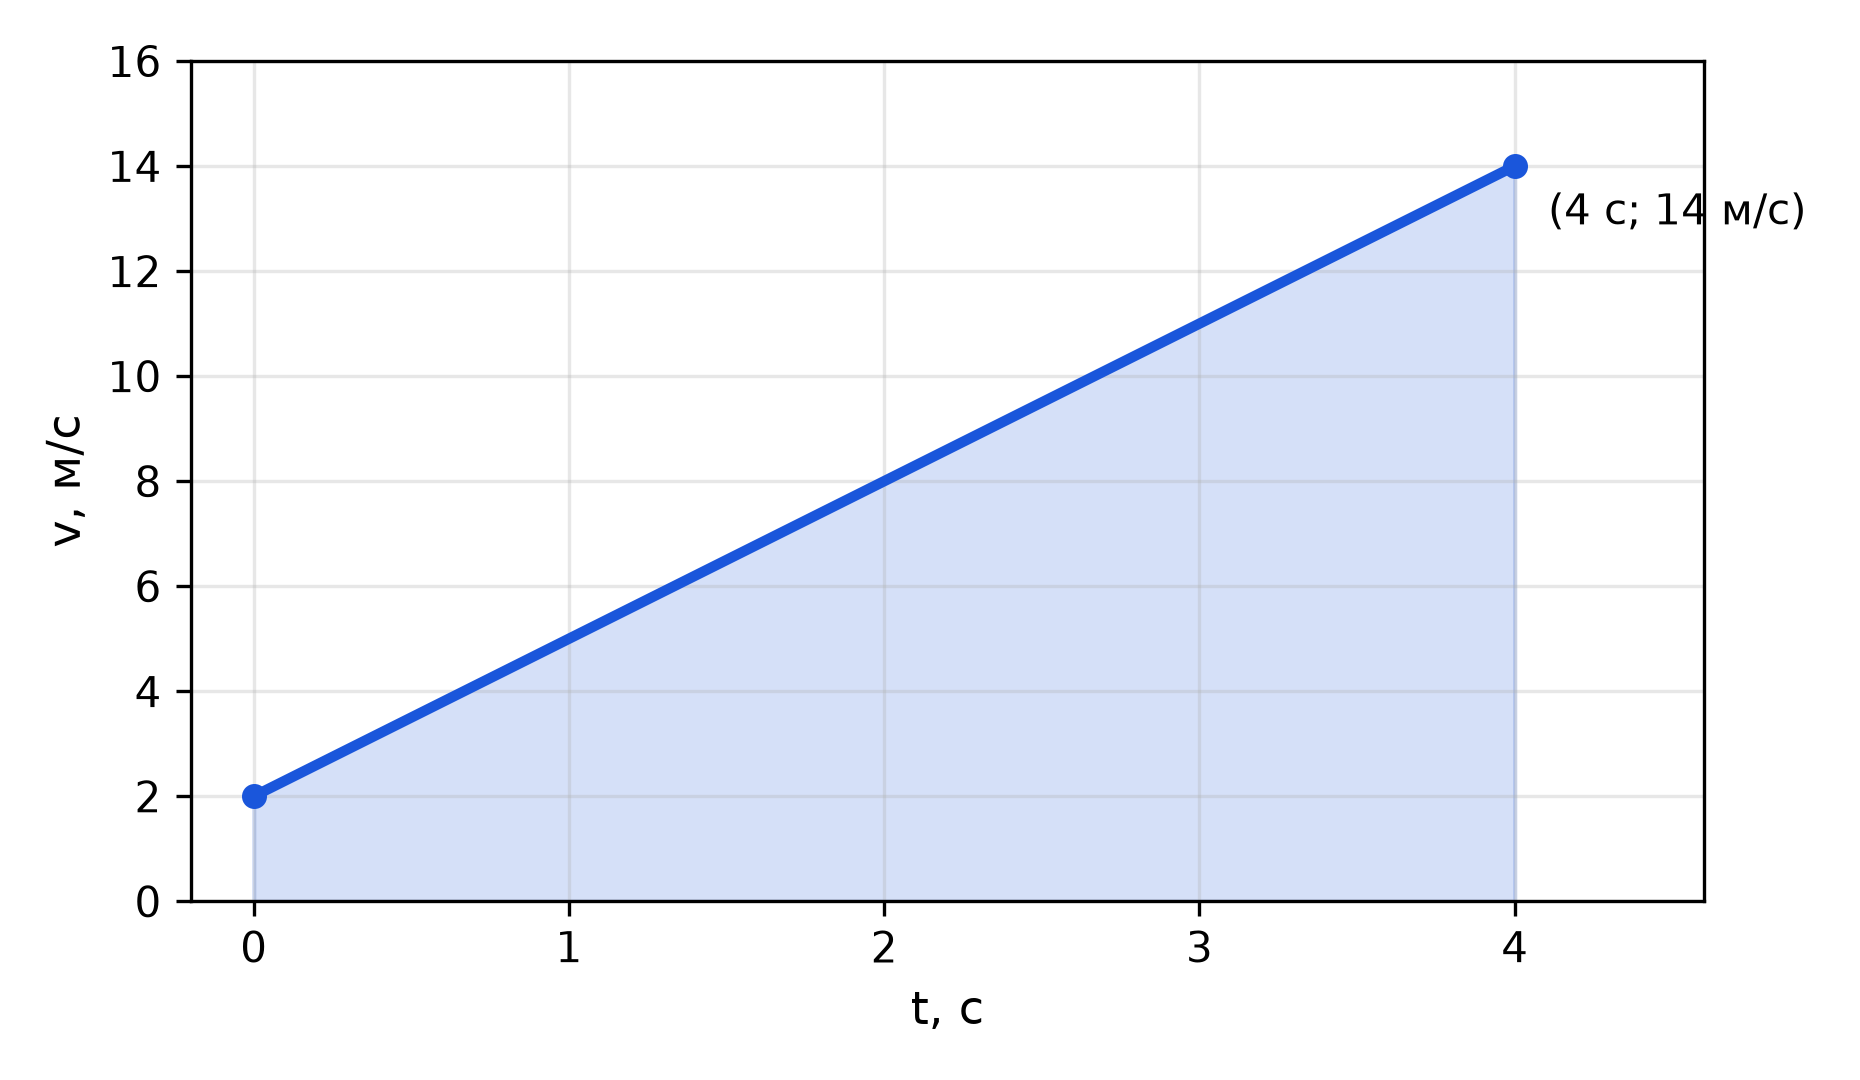
\includegraphics[width=0.85\textwidth]{fig_vt_kk.png}\caption{$v(t) = 2 + 3t$ графигі: түзудің көлбеуі — үдеу $a = 3$; боялған аудан — орын ауыстыру $s = 32$.}\end{figure}

\begin{figure}[htbp]\centering
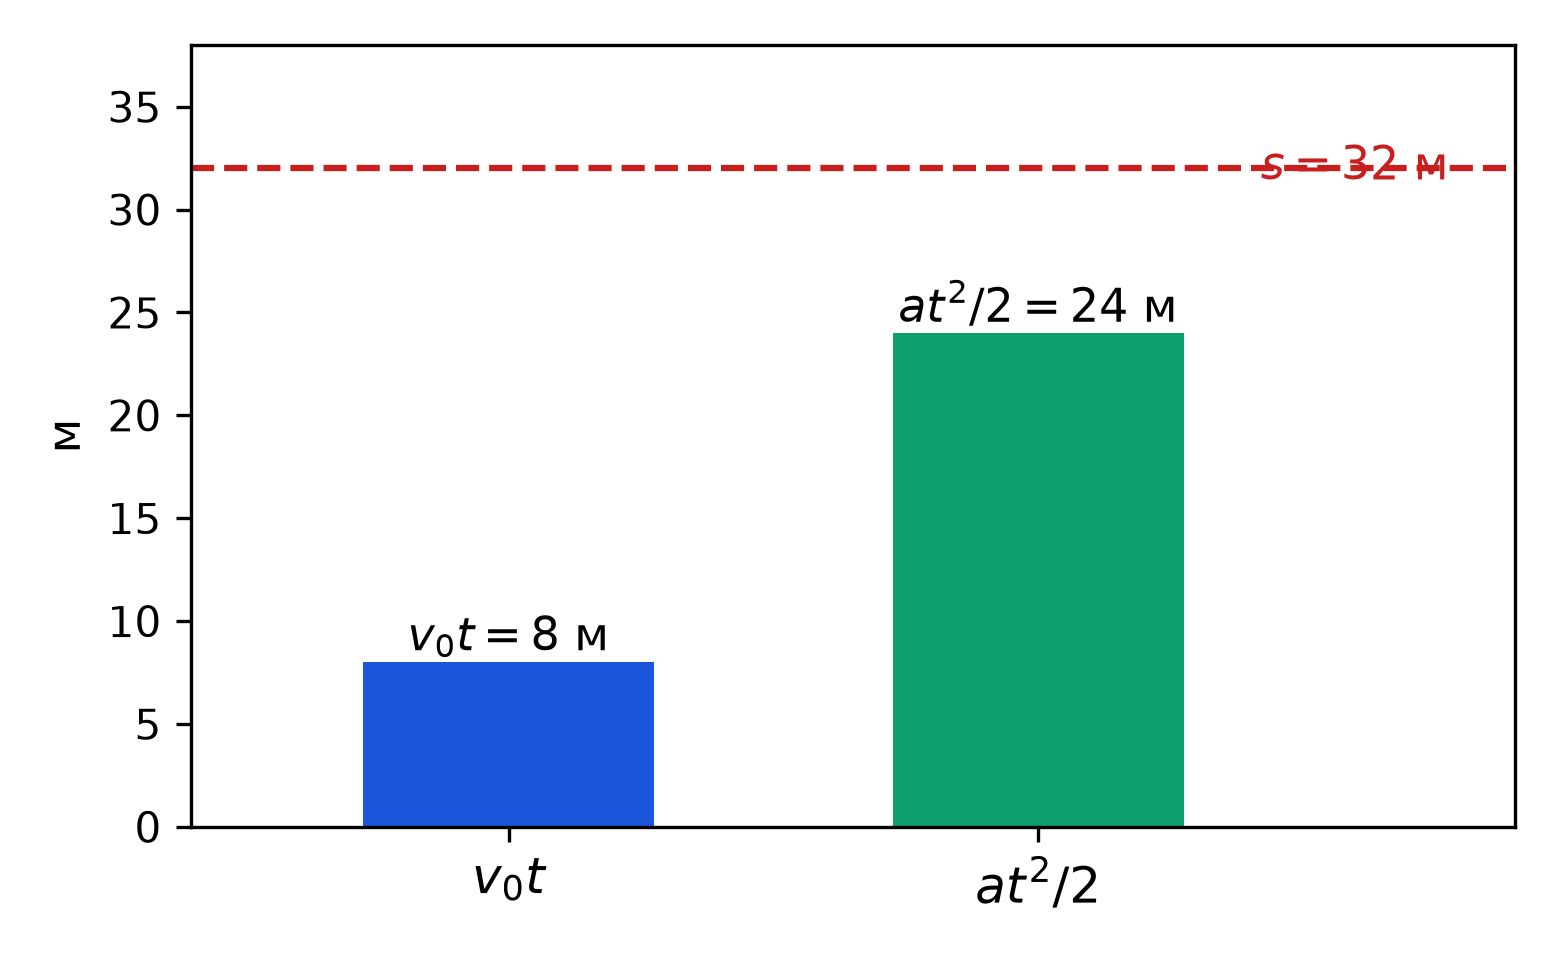
\includegraphics[width=0.7\textwidth]{fig_bars_kk.png}\caption{Орын ауыстыру екі қосылғышпен: $v_0t = 8$ плюс $at^2/2 = 24$; барлығы $s = 32$ м.}\end{figure}

\subsection*{Шығарылған мысал}
Берілгені: $v_0 = 2$ м/с, $a = 3$ м/с², $t = 4$ с. Табу керек: $v$, $s$.

\begin{enumerate}
\item $v = v_0 + at = 2 + 3\cdot 4 = 14$ м/с.
\item $s = v_0t + at^2/2 = 2\cdot 4 + 3\cdot 16/2 = 8 + 24 = 32$ м.
\item $s = (v_0+v)t/2 = (2+14)\cdot 4/2 = 32$ м.
\end{enumerate}
Бірліктерді тексеру: м/с² · с = м/с — сәйкес.

\subsection*{Қақпандар}
\begin{itemize}
\item Қақпан 1: $14\cdot 4 = 56$ — қате: жылдамдық өсті, орташасын алу керек.
\item Қақпан 2: көлбеу — бұл үдеу, аудан — орын ауыстыру.
\end{itemize}

\subsection*{Өздік тапсырмалар}
\begin{enumerate}
\item Дене 2 м/с бастапқы жылдамдықпен қозғалады. Оның үдеуі 3 м/с². 4 секундтан кейінгі жылдамдығын табыңыз.
\textbf{A)} 14 м/с \quad \textbf{B)} 12 м/с \quad \textbf{C)} 9 м/с \quad \textbf{D)} 6 м/с

\item Дене 2 м/с бастапқы жылдамдықпен, 3 м/с² үдеумен қозғалады. Бағыты өзгермесе, 4 с-тағы орын ауыстыруын табыңыз.
\textbf{A)} 32 м \quad \textbf{B)} 56 м \quad \textbf{C)} 24 м \quad \textbf{D)} 20 м

\item Қандай қозғалыс теңүдемелі деп аталады?
\textbf{A)} Жылдамдық тең уақыт аралықтарында бірдей шамаға өзгереді \quad \textbf{B)} Жылдамдық тұрақты \quad \textbf{C)} Үдеу уақыт өте келе өзгереді \quad \textbf{D)} Тең уақыт аралықтарында жол бірдей

\item Жылдамдықтың уақытқа тәуелділік графигіндегі түзудің көлбеуі нені көрсетеді?
\textbf{A)} Үдеуді \quad \textbf{B)} Орын ауыстыруды \quad \textbf{C)} Жылдамдықты \quad \textbf{D)} Уақытты

\item v(t) графигінде түзу (0 с; 2 м/с) нүктесінен (4 с; 14 м/с) нүктесіне барады. Орын ауыстыруды табыңыз.
\textbf{A)} 32 м \quad \textbf{B)} 48 м \quad \textbf{C)} 56 м \quad \textbf{D)} 24 м

\item Мәшине орнынан 2 м/с² үдеумен қозғалды. 5 с-та қанша жол жүреді?
\end{enumerate}
\newpage\subsection*{Жауаптар}
\begin{enumerate}
\item \textbf{A} — Үдеу жылдамдықты әр секунд сайын 3 м/с-қа арттырады. Сондықтан $v = v_0 + at = 2 + 3\cdot 4 = 14$ м/с.

\item \textbf{A} — $s = v_0t + at^2/2 = 2\cdot 4 + 3\cdot 16/2 = 8 + 24 = 32$ м. 56 м жауабы соңғы жылдамдықты бірқалыпты қозғалыс формуласына қойғанда шығады.

\item \textbf{A} — Теңүдемелі қозғалыста жылдамдық тең уақытта бірдей шамаға артады, үдеу тұрақты (Закирова 9, §3). D нұсқасы бірқалыпты қозғалысты сипаттайды.

\item \textbf{A} — v(t) графигінің көлбеуі үдеуге тең: $a = \Delta v/\Delta t$. Орын ауыстыру — график астындағы аудан (Закирова 10, §3).

\item \textbf{A} — Трапеция ауданы: $(2 + 14)/2 \cdot 4 = 32$ м. 24 м — тіктөртбұрышсыз тек үшбұрыштың ауданы.

\item \textbf{25 м} — $s = 0\cdot 5 + 2\cdot 25/2 = 25$ м.
\end{enumerate}

\subsection*{Дереккөздер}
Анықтамалар, формулалар мен график ережелері оқулықтармен салыстырылды; нөмірлер — PDF-беттер. Конспект тапсырмалары төл.
\begin{itemize}
\item Физика Закирова 9.pdf — анықтамалар мен формулалар кестесі: PDF с. 19–29.
\item Физика Закирова 10 ЖМ.pdf — графиктер мен аудан ережесі (§3): PDF с. 15–18, 20.
\item FBS (1).pdf — формулалар мен терминдерді салыстыру (Sailaubaev): PDF с. 6–7.
\item Testcenter -3.pdf — график ауданына ҰБТ есебінің форматы (1-есеп, 2-б.; B кілті, 37-б.): PDF с. 2, 37.
\item NCT physics sample (ru): \url{https://new.testcenter.kz/wp-content/uploads/2024/12/obr_var_test_02.pdf}
\item NCT physics sample (en): \url{https://new.testcenter.kz/wp-content/uploads/2025/06/PHYSICS.pdf}
\end{itemize}

Күйі: физика мен кілттер тәуелсіз тексерілді (G кезең); аударма мен терминдерді мұғалім тексеруі керек.
\end{document}
